\documentclass[twocolumn]{article}
\usepackage[fleqn]{mathtools}%for aligning parameters of fitted erfc(x)
\usepackage{geometry}	%
\usepackage{abstract} %to get email footnotes
\geometry{margin=2cm}	%more visible figures (more place) 
\usepackage[superscript,biblabel]{cite}%superscript citing
\usepackage[utf8]{inputenc}
\usepackage[english]{babel}
\usepackage{amsmath}	%booklet
\usepackage{hyperref}	%clickable citings, referencing URL via \url{}
\usepackage{siunitx}	%for SI units; see ftp://ftp.dante.de/tex-archive/macros/latex/exptl/siunitx/siunitx.pdf
\usepackage{graphicx} 	%includegraphics
\usepackage{mhchem}		%writing chemical elements with mass numbers
\usepackage[nottoc]{tocbibind}	%references
\usepackage{indentfirst}%indenting first paragraphs

%the command \insertFigure{file} inserts figure with width 0.9*(column width)
\newcommand{\insertFigure}[1]{%
   \includegraphics[width=0.95\linewidth]{#1}%
}

\title{\textbf{A248: Magneto-optical Trap}}
\author{Bence Mitlasóczki\thanks{s6bemitl@uni-bonn.de} and Beno\^it Scholtes\thanks{s6bescho@uni-bonn.de} \\ \textit{Rheinische-Friedrich-Wilhelms Universit\"at Bonn}}
\begin{document}
\renewcommand{\abstractname}{\vspace{-\baselineskip}} %supresses abstract title
\twocolumn[ %makes a one column abstract
\begin{@twocolumnfalse}
\maketitle

\begin{abstract} \vspace{-8mm}
We adjusted some mirrors to get MOT. We did some measurements.
\end{abstract}
\end{@twocolumnfalse}
\hspace{5mm} ]
\maketitle
\saythanks %from abstract package to ensure email footnotes from \thanks command in a two-column article
\section{Introduction}
Magneto-optical traps (MOT) are an important apparatus in modern atomic physics experiments, used to slow and trap a neutral atom cloud to temperatures as cold as several microkelvin. They are achieved by combining radiation pressure from laser beams and a quadropole magnetic field inside a vacuum cell rid of other gasses. Their use ranges from probing atomic properties, quantum optics, cold collision, quantum information processing, and acting as the preliminary stage to achieving even colder atom traps, namely Bose-Einstein condensates. This experiment aimed at obtaining a MOT and finding its size, population, and loading behaviour as well its fluorescence dependence on the magnetic field strength, quarter waveplate angle, and laser frequency detuning.

\section{Theory}
The central process by which atomic gasses are cooled are via radiation pressure from lasers. When a photon is absorbed by an object, particle, or atom, its energy as well as its momentum, equal to $p=\hbar k$, is absorbed as a result of momentum conservation. This radiation pressure can be used to slow down moving atoms if the atoms absorb photons travelling in the opposite direction. That said, only photons resonant to a transition of the absorption spectrum of the atoms are absorbed. As a result, the absorption spectrum of the atoms to be cooled needs to be known and a particular transition chosen such that the required frequency of the cooling laser can be determined.

%In order to obtain a MOT, two lasers are used. A cooling laser is used to actively slow and thus cool the atoms down, while a repumping laser is used to `repump' rare atoms that have excited to off-resonant states back into states that can be slowed by the cooling laser. The repumping laser will be explained in Section~\ref{sec:Rubidium}. Figure~\ref{fig:Laser} shows the setup for the preperation of the two lasers for the MOT.
%TODO talk about Doppler and natural broadening of spectrum, Voigt-profile
\subsection{Saturation Spectroscopy}
Atoms can only absorb photons with frequencies that are resonant to their excitation transitions. That said, a moving atom will not be able to absorb photons with these frequencies as their frequency will be Doppler shifted and no longer resonant to the atom transitions. The moving atom will only be able to absorb light which has been Doppler shifted such that it is resonant with one of its excitation transitions. In an uncooled gas, the atoms are all travelling in different directions with different speeds. As a result, light incident on the gas from one direction will be Doppler shifted differently for all the different atoms. An absorption spectrum obtained from such a gas will thus be Doppler broadened, making it difficult to determine the energy levels and transitions of the atoms. In order to obtain a spectrum with high resolution, Doppler-free spectroscopy such as saturation spectroscopy needs to be used. \\
\par Saturation spectroscopy makes use of two beams, often from the same source: the powerful pump beam and a weaker probe beam, passing through the sample in opposite directions. Due to the Doppler-broadened spectrum of the ensemble, there will be absorption in the wider frequency region for each beam, corresponding to a group of atoms (velocity class) which move with the right velocity in the beam direction.  As the frequency of the two beams matches, while their direction is opposite, the corresponding velocity classes move with velocities $\pm v$ along the common beam axis. If $v = 0$, that is, the laser frequency matches the transition frequency without doppler-shift, the probe beam shows a drop in the absorption signal (difference of original probe beam intensity and detected transmitted intensity), which is called the Lamb dip (a peak in the transmission spectrum). The narrowness of the Lamb dip compared to the Doppler-broadening allows for a much higher resolution.
An important phenomenon is the appearance of crossover peaks: these appear at the middle frequency of two close peaks with an intersection in their Doppler-broadened spectra. The two beams interact with the same velocity class, but producing the two different hyperfine transitions.

\subsection{Polarisation Spectroscopy}%Laser Spectroscopy p. 464 (485)
Polarization spectroscopy is based on saturation spectroscopy. The pump beam is circularly polarized by passing through a quarter waveplate before entering the sample. This can be shown to introduce anisotropy\cite{demtroder}$^{(\text{p.}\,465)}$ in the orientations of the angular momentum $J$ of the atoms, the sample becomes birefringent.
In the realised setup, the probe beam is split in two by a polarization beam splitter (PBS),
%TODO is PBS mentioned before?
only one of them passing through the anisotropic sample, turning its polarization axis slightly. After entering the detector, the difference of the signals is formed, which shows the axis shift. The result is a dispersive signal with a shape similar to what is shown on Figure \ref{fig:Dispersive}. The zero crossing with differing voltage signs on the two sides provides a precise locking point.
\begin{figure}
\centering
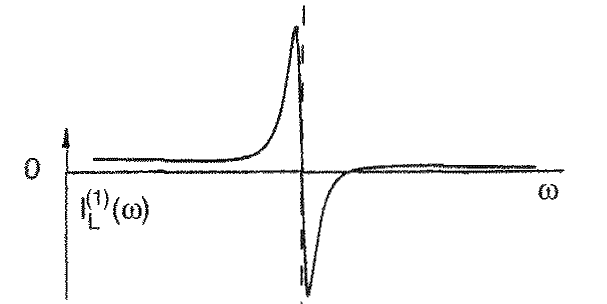
\includegraphics[scale=0.3]{Images/Dispersive.png}
\caption{A dispersive signal.\cite{demtroder}$^{(\text{p.}\,461)}$}
\label{fig:Dispersive}
\end{figure}
\subsection{Optical Cooling}

\subsection{Magneto-Optical Trap}
\subsubsection{Optical Trap}

\subsubsection{Magnetic Trap}

\subsection{Rubidium} \label{sec:Rubidium}
\begin{figure} [!h]
	\centering
	\insertFigure{Images/Spectrum.png}
	\caption{The dependency of MOT luminosity on the current flow through the coils and thus the strength of the magnetic field.}
	\label{fig:Spectrum}
\end{figure}
\iffalse
\begin{figure}[!h]
\centering
%\insertFigure{}
\caption{A sample figure}
\label{fig:example}
\end{figure}
\fi

\section{Experimental setup} \label{sec:Exp}
\begin{figure} [!h]
	\centering
	\insertFigure{Images/Laser.png}
	\caption{The dependency of MOT luminosity on the current flow through the coils and thus the strength of the magnetic field.\cite{manual}}
	\label{fig:Laser}
\end{figure}
\subsection{Diode Laser}
The lasers used in the experiment are diode lasers. The reason for using this type of lasers is for two reasons: first, the state transitions we exploit (cooling and repumping) lie in the infrared range (Figure \ref{fig:Laser}), second, we need tunable coherent light sources.\\
Recombination of an electron with a hole in a diode may result in electromagnetic radiation, with a large linewidth.\cite{demtroder} In the laser diode, the metal case for heat dissipation and optical cavity makes it possible that above a threshold current, population inversion can occur, which means lasing with a large free spectral range (below the threshold, the diode acts as a LED). The resonator modes can be shifted by changing the temperature (externally or by changing the diode current): the band gap, the index of refraction and the length of the cavity change. To use it in single mode, the laser is used in Littrow configuration, where an external grating is utilised. The grating is positioned such that for the desired frequency, the $-1.$ order is reflected back into the active medium, thus it serves as an external resonator element. The actual beam produced for use is the $0.$ order. For constructive interference, the grating equation reads\cite{demtroder}$^{(\text{p.}\, 114)}$ with the notation of Figure \ref{fig:Grating}:
\begin{equation}
2 d \sin \alpha = m \lambda\nonumber
\end{equation}
A piezo system functioning on triangular supply voltage is responsible for the moving of the grating, scanning through the laser spectrum.
\begin{figure}
	\centering
	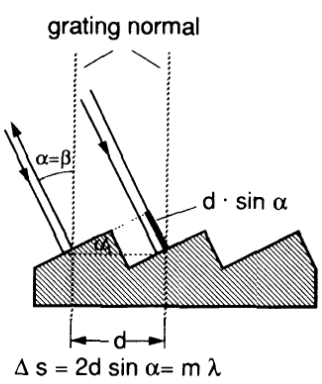
\includegraphics[scale=0.3]{Images/Grating.png}
	\caption{Diffraction grating in the special case when the incident and reflected beams coincide.\cite{demtroder}$^{(\text{p.}\, 114)}$}
	\label{fig:Grating}
\end{figure}
\begin{figure} [!h]
	\centering
	\insertFigure{Images/Diode.png}
	\caption{The diode laser with the grating in Littrow configuration.\cite{manual}}
	\label{fig:Diode}
\end{figure}
\subsection{Laser Detuning}

\subsection{MOT setup}
\begin{figure} [!h]
	\centering
	\insertFigure{Images/MOT.png}
	\caption{The MOT setup.\cite{manual}}
	\label{fig:MOT}
\end{figure}

\section{Procedure} \label{sec:Proc}

\section{Measurements}

\subsection{Laser beam diameter}
Using a movable razor blade and a powermeter, we measured the intensity as a function of the displacement of the blade along an axis perpendicular to the beam propagation direction. The results are collected in Table \ref{table:beampower}. Fitting a function of the form
\begin{alignat*}{2}\label{erf}
f(x) &= \mathrlap{P + A \cdot \text{erfc}(B\cdot x - C),}
\shortintertext{we found}
P &= & 0.012 \pm 0.009,\\
A &= & 0.735 \pm 0.007,\\
B &= & 4.942 \pm 0.133,\\
C &= & 198.039 \pm 5.317.
\end{alignat*}
%TODO Any units for these values? Remember these values are still inside a sentence, so proper punctuation is still necessary.
\begin{table}
\centering
\begin{tabular}{|c|c|}
\hline
Position (cm)	& Power (mW)\\
\hline
$39.4 \pm 0.05$	&	$1.58 \pm 0.01$\\ 	\hline
$39.5 \pm 0.05$	&	$1.57 \pm 0.01$\\ 	\hline
$39.6 \pm 0.05$	&	$1.52 \pm 0.01$\\ 	\hline
$39.7 \pm 0.05$	&	$1.40 \pm 0.01$\\ 	\hline
$39.8 \pm 0.05$	&	$1.07 \pm 0.01$\\ 	\hline
$39.9 \pm 0.05$	&	$0.62 \pm 0.01$\\ 	\hline
$40.0 \pm 0.05$	&	$0.25 \pm 0.01$\\ 	\hline
$40.1 \pm 0.05$	&	$0.10 \pm 0.01$\\ 	\hline
$40.2 \pm 0.05$	&	$0.04 \pm 0.01$\\	\hline
$40.3 \pm 0.05$	&	$0.01 \pm 0.01$\\	\hline
$40.4 \pm 0.05$	&	$0.00 \pm 0.01$\\	\hline
\end{tabular}
%TODO last value can be negative within that error range, fix that maybe? These uncertainties need to be much larger, we saw a lot more deviations for these during measurement taking. I guess we'll estimate some kind of relative error for all of these to pretend we actually quantified uncertainty then and there. The last point could have zero negative uncertainty (+0.01, -0.00).
\caption{Beam power as a function of position of the razor blade. Clearly visible}
\label{table:beampower}
\end{table}
This results in a width %http://people.fjfi.cvut.cz/blazejos/public/ul7en.pdf
\begin{equation}
w = 0.2860 \text{ cm } \pm 0.0077 \text{ cm} \nonumber
\end{equation}
\subsection{Size of MOT}
\begin{figure}
\centering
\insertFigure{Images/MOT_w_scale_crop.png}
\caption{Photo of the MOT merged with photo of the scale.}
\label{fig:mot_w_scale}
\end{figure}
%TODO Crop slightly to make the MOT more visible/central
To get an estimate on the MOT size we took a picture of, we used a scale put in the focus to convert distances in pixels to centimeters. By choosing two points $\SI[separate-uncertainty = true]{30.0 \pm 0.5 }{\milli\meter}$ from each other in the image (the error due to the width of the millimeter lines on the scale and the two points not at the same distance from the edge of the ruler), the image viewer software showed $742.2$ pixels. Then
\begin{equation}
1 \text{~px} = \SI[separate-uncertainty = true]{40.42 \pm 0.67}{\micro\meter} \nonumber
\end{equation}
As visible on Figure \ref{fig:mot_w_scale}, the MOT has different horizontal and vertical size values. The directly measured width and height for the MOT are
\begin{align*}
h &= (72 \pm 2)  \, \text{px}\\
w &= (57 \pm 2)  \, \text{px} 
\end{align*}
We chose to approximate the volume by an ellipsoid with one axis half the height ($c$) and two axes half the width ($a$, $b$) each.
\begin{align*}
a, b &= \SI[separate-uncertainty = true]{1.15 \pm 0.04}{\milli\meter} \\
c &=  \SI[separate-uncertainty = true]{1.46 \pm 0.05}{\milli\meter} \\
V &= \frac{4}{3} \pi a b c = \SI[separate-uncertainty = true]{8.09 \pm 0.52 }{\cubic\milli\meter}
\end{align*}
\subsection{Changing the magnetic field}
To measure the MOT fluorescence as a function of the magnetic field, we changed the current flowing through the coils. Figure \ref{fig:magnetic} shows our results. To get a visible MOT, we had to set the current to a minimal value of around $0.9$ A, below this the system fails to trap the moving atoms; from this point, the fluorescence grew proportional to the current to a good approximation, up to $4.6$ A. The background fluorescence has been previously measured and substracted from the data.
\begin{figure}
\centering
\insertFigure{Images/magnetic_dependence_wo_linear.png}
\caption{The dependency of MOT luminosity on the current flow through the coils and thus the strength of the magnetic field.}
\label{fig:magnetic}
\end{figure}
%TODO What is the dependence of the magnetic field with current flow? Should we investigate this or not?
\subsection{Loading behaviour}
\begin{figure}
\centering
\insertFigure{Images/mot_buildup.png}
\caption{Example of data points exported from the oscilloscope, with fitted function (red).}
\label{fig:buildup}
\end{figure}
After replacing the powermeter with a photodiode and showing its signal on an oscilloscope, we used the data from 6 MOT buildup events to find the loading time. As it is known,\cite{inexpensive} the number of trapped atoms changes as
\begin{equation}\label{eq:load}
N(t) = N_0 \big( 1 - e^{-\frac{t}{\tau}} \big),
\end{equation}
where $\tau$ is the loading time, $N_0$ is the maximal number of atoms in the trap. The cross-section is related to $\tau$ if there is only $\ce{Rb}$ in the vacuum chamber (which we assume):
\begin{equation}\label{eq:cross-section}
\frac{1}{\tau} = n_{\text{Rb}} \sigma_{\text{Rb}} v_{\text{Rb}},
\end{equation}
where $n_{\text{Rb}}$ is the number density, $v_{\text{Rb}}$ is the average velocity of the $\ce{Rb}$ vapor (in the following, the subscript Rb is ignored).\\
As the luminescence-time signal also follows Eqn. \ref{eq:load}, by fitting such a function to the oscilloscope data we have gathered yields $\tau$:
\begin{equation}
\tau = (0.268 \pm 0.006) \, \text{s}\nonumber
\end{equation}
With the recorded temperature $T = (293.55 \pm 0.05) \, K$ and pressure $p = (8.09 \pm 0.01)\cdot 10^{-8} \, \text{mbar}$,
%mass of 85 Rb: 84.911 amu = 141.037*10^-27 kg
\begin{equation}
v = \sqrt{\frac{2kT}{m}} = (293.545 \pm 0.025) \, \frac{\text{m}}{\text{s}} \nonumber
\end{equation}
The number density $n$ can be calculated from the ideal gas law:
\begin{equation}
n = \frac{N}{V} = \frac{p}{kT} = (1.99704 \pm 0.00250)\cdot 10^{15} \, \frac{1}{\text{m}^3}\nonumber
\end{equation}
Finally, the cross-section:
\begin{equation}
\sigma = \frac{1}{n \tau v} = (6.355 \pm 0.131) \cdot 10^{-18} \, \text{m}^2
\end{equation}
\section{Conclusion}

\begin{thebibliography}{9}
\bibitem{inexpensive}
C. Wieman, G. Flowers and S.Gilbert, Am. J. Phys. \textbf{63} (1995).
\bibitem{manual}
Unspecified Author, \textsl{FP Experiment: Rubidium MOT} (University of Bonn, 2014).
\bibitem{metcalf}
H. Metcalf and P. van der Straten, \textsl{Laser Cooling and Trapping} (Springer, 1999).
\bibitem{demtroder}
W. Demtröder, \textsl{Laser Spectroscopy, Basic Concepts and Instrumentation} (Springer, 2003).%Third Edition
\bibitem{laserdiode}
\textsl{Physics Fundamentals: Laser Diode Characteristics}, \url{https://www.sukhamburg.com/download/fundamentals-laserdiodes.pdf}
\iffalse
%Leaving this here as examples for referencing different media
\bibitem{book}
K. Siegbahn, \textsl{Alpha-, beta-, and gamma-ray spectroscopy, Vol. 2} (North Holland Publishing Company, Amsterdam, 1965).
\bibitem{booklet}
Unspecified author, \textsl{Advanced Laboratory Course (physics601): Description of Experiments} (University of Bonn, 2018).
 \bibitem{link}
 W. U. Boeglin, \textit{Scintillation Detectors}, WWW Document, \url{http://wanda.fiu.edu/teaching/courses/Modern_lab_manual/scintillator.html}.
\bibitem{pdf_on_website}
Unspecified author, \textsl{Gamma Ray Spectroscopy} (University of Florida, 2013), \url{https://www.phys.ufl.edu/courses/phy4803L/group_I/gamma_spec/gamspec.pdf}.
\bibitem{cfd}
E. Ermis and C. Celiktas, International Journal Of Instrumentation Science 1, (2013), pp.54-62.
%alternative url: https://en.wikipedia.org/wiki/Constant_fraction_discriminator
\bibitem{signal}
M. Nakhostin, \textsl{Signal Processing for Radiation Detectors} (John Wiley $\&$ Sons, 2018), p. 298\footnote{Relevant pages (chapter 6) available for preview under\\ \url{https://books.google.de/books?id=Lrg4DwAAQBAJ}}.
%Mohammad Nakhostin
\bibitem{leo}
W. R. Leo, \textsl{Techniques for Nuclear and Particle Physics Experiments} (Springer-Verlag, 1987), p. 305.
%William R. Leo
\bibitem{meliss}
A. C. Melissinos, J. Napolitano, \textsl{Experiments in Modern Physics, 2\textsuperscript{nd} edition} (Academic Press, San Diego, 2003), pp 419-21.
\fi
\end{thebibliography}
\end{document}